\documentclass{article}
\usepackage{apacite}
\usepackage{graphicx}
\graphicspath{ {./} }
\usepackage{amssymb}
\usepackage{mathtools}
\usepackage{multicol}
\title{\textbf{{\large LU3IN013}\\Research Project}\\{\Huge Formal Modeling of Algorithms\\for Distributed Systems}\\\textit{First Report}}
\author{\Large\textbf{Tra My Nguyen}\\{\large 3702069}}
\date{\textit{2019-2020}}

\begin{document}
	
	\maketitle
	\pagenumbering{arabic}
	\newpage
	
	\section{Introduction}
	
	\subparagraph{}Distributed systems are omnipresent nowadays as they help resolving various computing problems with efficiency and high adaptability. However, along these advantages come a lot of difficulties due to the fact that entities in these systems run concurrently and can only communicate with each other via message-passing. As a result, coordinating the behavior of independent components of the system becomes the major challenge in distributed computing and one that is really hard to analyze. Instead of relying on traditional extensive testing, modern day system design uses formal methods based on mathematical techniques to study the reliability and robustness of a system. One proposal is the Carl Adam Petri's seminal work on Petri nets in the early 1960s.
	\subparagraph{}This project is carried out in responding to the Call for Models by the Model Checking Contest handled annually by LIP6, an event where formal verification tools for concurrent systems are evaluated in order to find the best suited techniques for a class of problem (e.g. state space generation, deadlock detection, reachability analysis, causal analysis). The goal is to create formal models with scaling capabilities from distributed algorithms using previously mentioned Petri nets, which may then be used alongside others in the contest as common benchmarks on which all tools will be compared.
	\subparagraph{}In this first report, I will be giving a general view on the notion of Petri nets and their functioning principle, as well as an initial application of Petri nets in modeling a Client-Server communication system. I will also be briefly presenting two distributed algorithms from which I will attempt to create Petri nets models and the steps I will take to work toward that goal.
	
	\section{Petri Net}
	\subparagraph{}Place/Transition Petri nets (P/T net) will be the main focus in this project.
			
	\begin{center}
		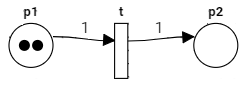
\includegraphics[scale=0.6]{net1}
		\\Figure 1: An simple P/T net
	\end{center}
	\subparagraph{}
	The image above shows \textbf{a place/transition net (P/T net)}, which, at first glance, resembles a bipartite oriented weighted graph. Its vertices can be separated into a set of rectangle (known as transitions) and a set of circles (places), each circles containing a number of dots (tokens). A state of a P/T net is established by the number of tokens held by each place, formally defined by a marking. Transitions of a P/T net represent actions that can take place and modify its state. The cost of one action is indicated on its input arc (number of tokens taken away from the source place) and its product on the output arc (number of tokens added to the target place).
	\subparagraph{}The models to be produced in the project need to be scalable, which means by increasing a certain type of actors having similar behaviors in a system (parameters), we obtain multiple P/T nets describing the same scenario but of different sizes (number of transitions/places/arcs) or of different initial marking.
	\subsection{Formal definitions}
	\subparagraph{}A P/T net can be hereby formally defined as\textit{ a tuple} $\mathcal{N} = (P,T,\textbf{Pre},\textbf{Post}),$ \textit{where
		\\$\bullet$ P is a finite set of \underline{places}, representing resources in a system, each place holds a number of \underline{tokens}, representing the number of occurrences of a resource
		\\$\bullet$ T is a finite set of \underline{transitions}, disjoint from P, representing actions that can occur in the system, and} 
		\\$\bullet$ \textbf{Pre},\textbf{Post} $\in\mathbb{N}^{|P|\times|T|}$ \textit{are matrices (the backward and forward incidence matrices of $\mathcal{N}$), \textbf{C} $=$ \textbf{Post} $-$ \textbf{Pre} is called the incidence matrix of $\mathcal{N}$.}
	\begin{table}[h]
		\begin{center}
			\begin{tabular}{ |c|c| } 
				\hline
				\textbf{Pre} & \textit{t}\\
				\hline
				$\textit{p}_{1}$ & 1\\ 
				$\textit{p}_{2}$ & 0\\ 
				\hline
			\end{tabular}
			%
			\begin{tabular}{ |c|c| } 
				\hline
				\textbf{Post} & \textit{t}\\
				\hline
				$\textit{p}_{1}$ & 0\\ 
				$\textit{p}_{2}$ & 1\\ 
				\hline
			\end{tabular}
			%
			\begin{tabular}{ |c|c| } 
				\hline
				\textbf{C} & \textit{t}\\
				\hline
				$\textit{p}_{1}$ & -1\\ 
				$\textit{p}_{2}$ & 1\\ 
				\hline
			\end{tabular}
			\caption{The incidence matrices of the P/T net in Figure 1}			
		\end{center}
	\end{table}
	\\A marking of a P/T net $\mathcal{N} = (P,T,\textbf{Pre},\textbf{Post})$ is a vector $\textbf{m}\in\mathbb{N}^{|P|}$. $\mathcal{N}$ \textit{together with a marking }$\textbf{m}_{0}$ \textit{(initial marking) is called} \textbf{a P/T net system} $\mathcal{S} = (\mathcal{N},\textbf{m}_{0})$. 
	\subparagraph{}It can be said that \textit{a transition $\mathit{t}\in\mathit{T}$ is enabled in a marking $\mathbf{m}$ if $\mathbf{m}\geq\mathbf{Pre}[\bullet,\mathit{t}]$. In this case } \textbf{the successor marking relation} \textit{is defined by $\mathbf{m}\xrightarrow{t}\textbf{m}'\Leftrightarrow \mathbf{m}\geq\mathbf{Pre}[\bullet,t]\land\mathbf{m}'=\mathbf{m}+\mathbf{Post}[\bullet,t]-\mathbf{Pre}[\bullet,t]=\mathbf{m}+\mathbf{C}[\bullet,t]$ ($\mathbf{Pre}[\bullet,t]$ denotes the t-column vector $ \mathbf{Pre}[\bullet,\mathit{t}]=(\mathbf{Pre}[p_{1},t],...,\mathbf{Pre}[p_{|P|},t])$) of the $|P|\times|T|$ matrix $\mathbf{Pre}$. The same holds for $\mathbf{Post}[\bullet,t]$ with respect to $\mathbf{Post}$.}
	\subparagraph{}Here, the initial marking is $\mathbf{m}_{0}=[2,0]>\mathbf{Pre}[\bullet,t]=[1,0]$, the transition \textit{t} is therefore fireable and firing it will lead to the successor marking $\mathbf{m}_{1}=[1,1]$.
	\begin{center}
		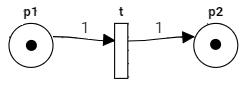
\includegraphics[scale=0.6]{net}
		\\Figure 2: New P/T net after firing transition $t$
	\end{center}
	\section{An example: Client-Server System}
	\subparagraph{}Let's look at the example of an P/T net simulating a communication channel between 2 clients and 2 servers. Each client can send a request to the channel, which will address the request to one of the servers and transfer the reply back to the same client once the chosen server has responded.
	\begin{center}
		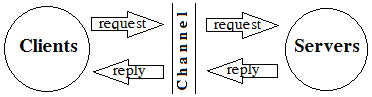
\includegraphics[scale=0.7]{cssys}
		\\Figure 3: Client-Server communication system
	\end{center}
		\textbf{Places}:
		\\\underline{Channel}
		\\$\bullet$ \texttt{sys}, waiting for request
		\\$\bullet$ \texttt{sys\_req$_{i}$}, having request from Client$_i$
		\\$\bullet$ \texttt{sys\_rep$_{i}$}, having reply for request of Client$_i$
		\\
		\underline{Client$_i$}
		\\$\bullet$ \texttt{c$_i$}, wanting to send request
		\\$\bullet$ \texttt{ca$_i$}, waiting for reply
		\\
		\underline{Server$_i$}
		\\$\bullet$ \texttt{sv$_i$}, available
		\\$\bullet$ \texttt{sv$_i$\_c$_j$}, treating request from Client$_j$
		\\\\\textbf{Transitions}:
		\\\underline{Channel and Client$_i$}
		\\$\bullet$ \texttt{send$_i$}, Client$_i$ sending request to channel
		\\$\bullet$ \texttt{receive$_i$}, Client$_i$ receiving reply from channel
		\\\underline{Server$_i$}
		\\$\bullet$ \texttt{req$_i$\_c$_j$}, receiving request of Client$_j$ from channel
		\\$\bullet$ \texttt{rep$_i$\_c$_j$}, sending reply to request of Client$_j$ to channel
		\\\\

	\begin{center}
		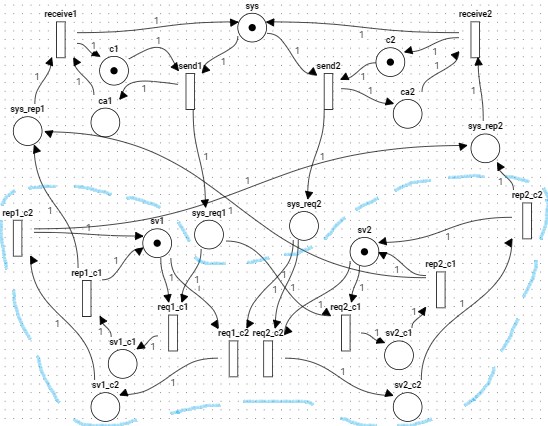
\includegraphics[scale=0.75]{cl2sv2}
		\\Figure 4: P/T net of 2 Clients and 2 Servers system
	\end{center}
	It can be seen that for a given server, there is only one token in the initial marking and there are as many sets of \{sv$_i$\_c$_j$,req$_i$\_c$_j$,rep$_i$\_c$_j$\} as there are clients, for the reason being that a server can take a request from any client and while processing that request, it is no longer available. The channel also processes one request at a time and a client can only send one request at a time. Since the set of places and transitions of all Server$_i$ is transition-bordered (only transitions in the set are linked to the rest of the model), it can be abstracted into one common transition like in the following P/T net.
	\begin{center}
		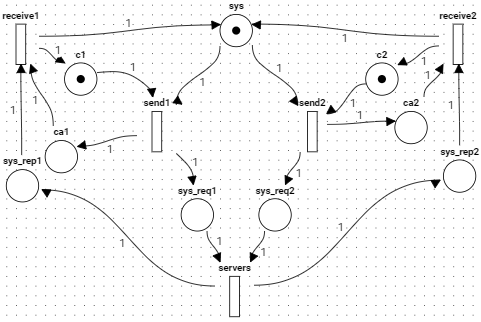
\includegraphics[scale=0.72]{cl2sv2abs}
		\\Figure 5: Abstracted P/T net of 2 Clients and 2 Servers system
	\end{center}
	\section{Algorithms}
	\subparagraph{}Firstly, I will be looking at a classic problem in a distributed system: leader election, where node with the highest identity number in a network would be elected as the leader. The algorithm below, presented by D.S.Hirschberg and J.B.Sinclair(1980), shows the procedure of each node in a bidirectional ring network (where each node of identity $id_{i}$ has two neighbors $left_{i}$ and $right_{i}$ with whom it can communicate (send and receive messages)). 
	\\I will be modeling the behavior of each node, how they react to a message from another node. All nodes will receive a START message from exterior. Each node then sends ELECTION($id_{i},0,1$) to both of its neighbors, presenting its own identity, the first round number $r=0$ and the number of nodes its message has visited $d=1$. During each round \textit{r}, each node competes with its $2^{\mathit{r}}$ neighbors to the left and to the right, and only the winner of round \textit{r} can continue to round $\mathit{r}+1$. After one round, the identity of the winner of a neighborhood will be sent in a REPLY message back to the winner itself, a node receiving two REPLY messages from both sides learns that it is the winner of its $(2^{r}+1)$ neighborhood and moves on to the new round. The process ends with the node of highest identity number sending an ELECTION message to itself and becoming the leader, and then, all nodes learning the identity of the leader thanks to the ELECTED message.
		\begin{center}
			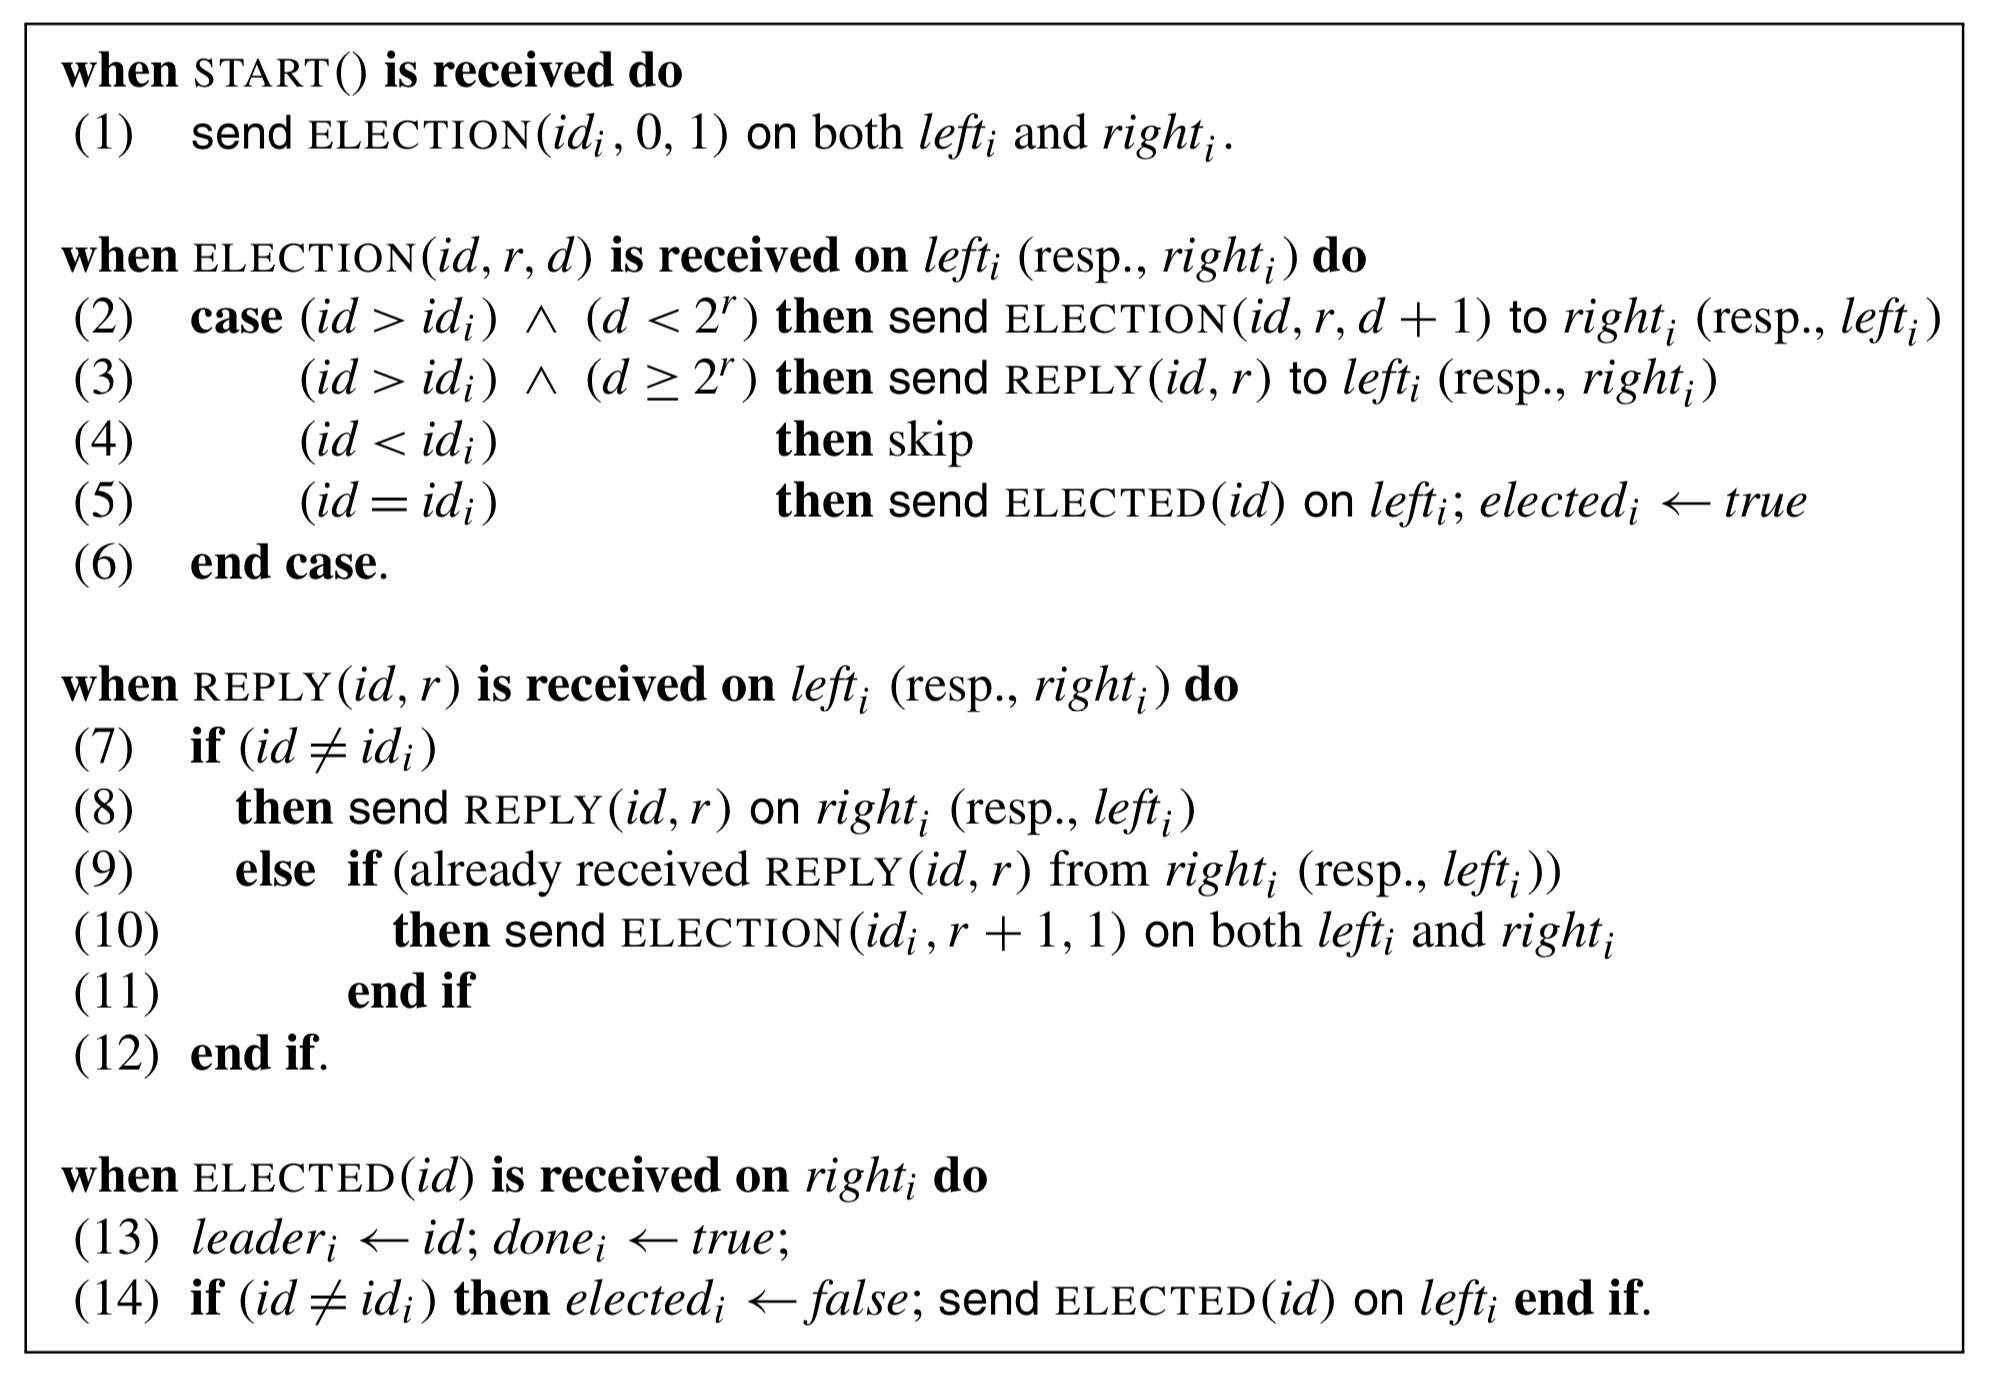
\includegraphics[scale=0.17]{IMG_7599}
			\\Figure 6: Leader election algorithm for bidirectional ring network			
		\end{center}
	\subparagraph{}Secondly, I will turn to an algorithm that I have studied in the sequential context: Bellman-Ford's Shortest Path Algorithm, and try to model its distributed adaptation. The goal is that each vertex in a non-oriented weighted graph learns the shortest path from itself to every other vertex. It is based on the principle of dynamic programming where each vertex $p_{j}$ stores an array $length_{i}[1..n]$ such that $length_{i}[k]$ will contain the length of the shortest path from $p_{i}$ to $p_{k}$ (initially, $length_{i}[i]=0$ and $length_{i}[k]=+\infty$ for $k \neq i$). When a node $p_{i}$ updates its $length_{i}$ (by comparing the length of the newly learned and the old path and updating if the new path is shorter), it will signal all of its neighbors $p_{j}$ to update their own $length_{j}$ array. For a node $p_{i}$, $l_{g_{i}}[j]$ denotes the length associated with the channel $(i,j)$ and $routing\_to_{i}[1...n]$ is such that $routing\_to_{i}[k]=j$ means that $p_{j}$ is a neighbor of $p_{i}$ on a shortest path to $p_{k}$. The algorithm ends when each node acquires the knowledge of the shortest path to other nodes, there will not be anymore UPDATE message as the condition in which $update_{i}$ becomes $true$ can no longer be satisfied.
		\begin{center}
			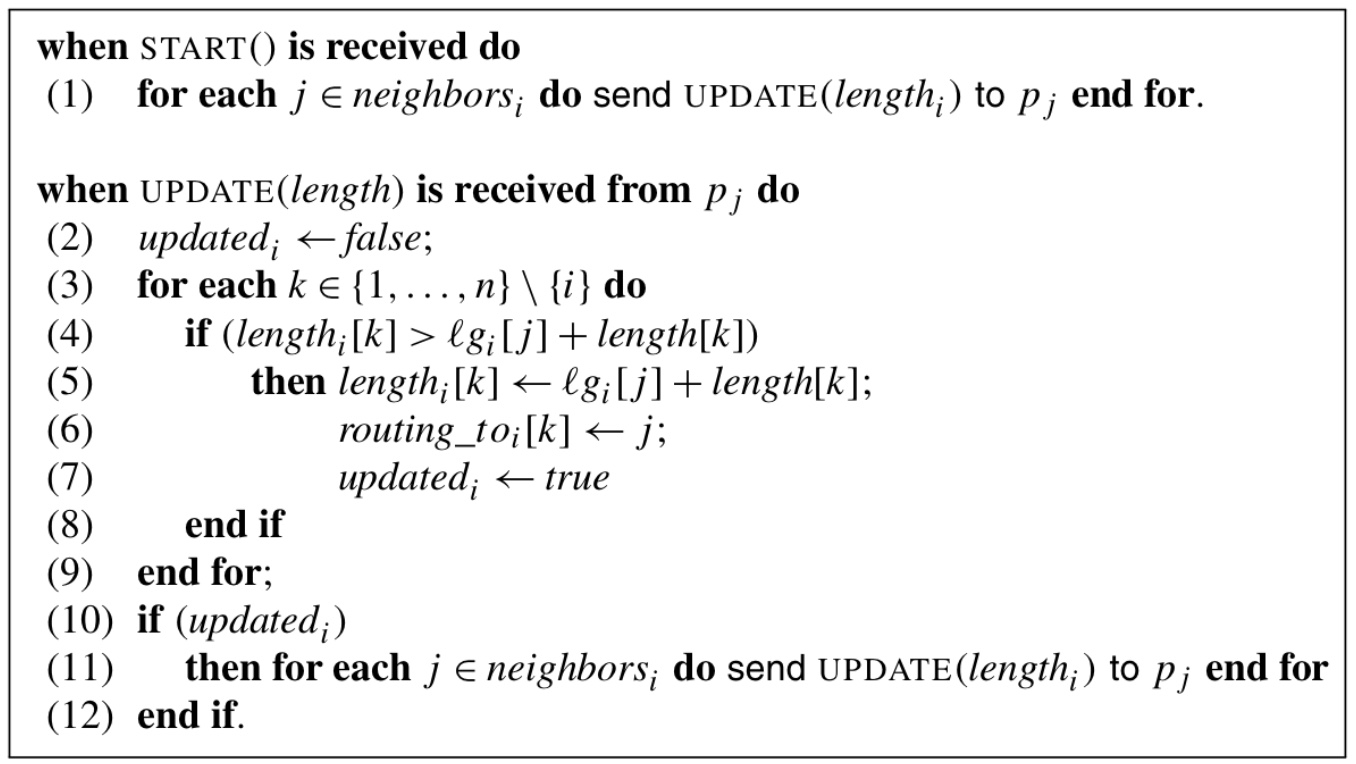
\includegraphics[scale=0.25]{IMG_7653}
			\\Figure 5: Distributed adaptation of Bellman-Ford's Shortest Path algorithm
		\end{center}
	\section{Conclusion}
	\subparagraph{}For the next step of the project, I will be working with the PNML Framework library implemented in Java, which allows creating models in PNML format required by the MCC. The first model will be the continuation of the Client-Server problem, by developing a generator which puts together pieces of each type of actor in the communication scenario, I can obtain Client-Server models of different scales. Once having mastered the basis of the library, I will begin modeling the above-mentioned algorithms, starting with analyzing them. By looking at the characteristics of these algorithms, I will be able to identify their scaling capabilities (for example here, the amount of nodes/vertices), the interactions of interest between elements of the algorithms and all the possible scenarios. After that, by producing multiples models, I hope to be able to provide the MCC with some interesting ones. 
\bibliographystyle{apacite}
\bibliography{bibpjrech}
\end{document}